\section{Collaboration}

\begin{frame}
  \tableofcontents[currentsection]
\end{frame}

\begin{frame}{Collaboration}
  \begin{itemize}
    \item Jedes git Repository enthält die vollständige Versionshistorie
    \item Jeder Benutzer kann Repositories veröffentlichen (push)
    \item Unterstützte Protokolle:
    %http://progit.org/book/ch4-1.html
    \begin{itemize}
      \item file
      \item git
      \item http(s)
      \item ssh
    \end{itemize}
    \item Git unterstützt mehrere Entwicklungsmodelle (Distributed Workflows)
  \end{itemize}
\end{frame}

\begin{frame}
  \begin{figure}
    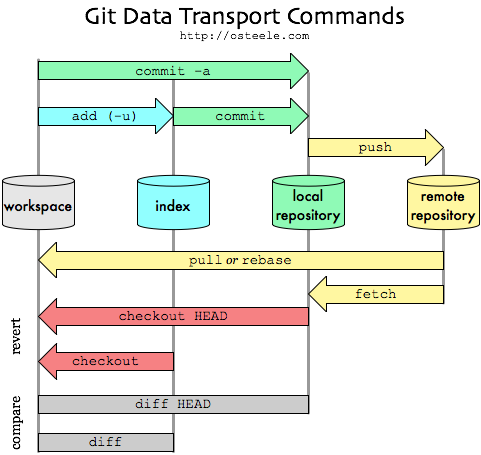
\includegraphics[width=0.5\textwidth]{img/git-transport}
    \caption[format=empty]{Quelle: \url{http://osteele.com/archives/2008/05/my-git-workflow}}
  \end{figure}

\end{frame}

\begin{frame}{Distributed Workflows}
  \framesubtitle{Centralized Workflow}
  \begin{figure}
    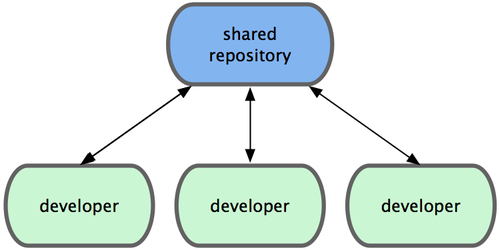
\includegraphics[width=0.5\textwidth]{img/wf-centralized}
    \caption[format=empty]{Quelle: \url{http://progit.org}}
  \end{figure}
\end{frame}

\begin{frame}{Distributed Workflows}
  \framesubtitle{Integration-Manager Workflow}
  \begin{figure}
    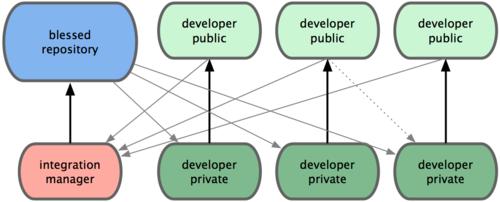
\includegraphics[width=0.6\textwidth]{img/wf-integration-manager}
    \caption[format=empty]{Quelle: \url{http://progit.org}}
  \end{figure}
\end{frame}

\begin{frame}{Distributed Workflows}
  \framesubtitle{Dictator and Lieutenants Workflow}
  \begin{figure}
   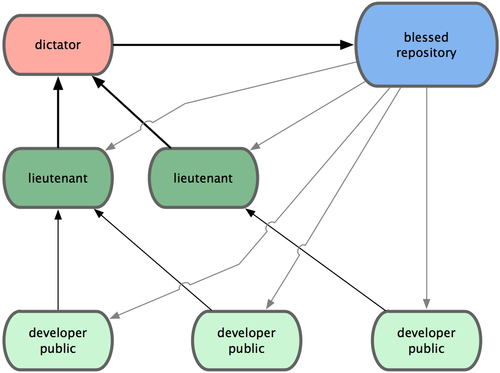
\includegraphics[width=0.5\textwidth]{img/wf-dictator}
    \caption[format=empty]{Quelle: \url{http://progit.org}}
  \end{figure}
\end{frame}

\begin{frame}[allowframebreaks]{Git Hosting}
  \begin{itemize}
    \item Github:
    \begin{itemize}
      \item Hosting unter: \url{http://github.com}
      \item Hohe Popularität
      \item Viele Features
      \item Quellcode nicht verfügbar
    \end{itemize}
    \item Gitorious:
    \begin{itemize}
      \item Hosting unter: \url{http://gitorious.org}
      \item Integrierte Benutzerverwaltung
      \item Freie Software (AGPL, \url{http://gitorious.org/gitorious})
    \end{itemize}
  \framebreak
    \item Gitosis:
    \begin{itemize}
      \item Einfach, gut geeignet für kleineres Setup
      \item Freie Software (GPLv2, \url{http://eagain.net/gitweb/?p=gitosis.git})
    \end{itemize}
    \item Gitolite:
    \begin{itemize}
      \item Komplex, aber sehr flexibel
      \item Freie Software (GPLv2, \url{https://github.com/sitaramc/gitolite})
    \end{itemize}
  \end{itemize}
\end{frame}

\begin{frame}[fragile]{Git Repositories klonen}
  \begin{itemize}
    \item Git kopiert beim Klonen immer die vollständige Versionshistorie
    \item Die Adresse des geklonten Repositories wird automatisch mit dem Namen „origin“ angelegt
    \item Die Quellen dieses Workshops klonen:
    \begin{lstlisting}
$ git clone git://gitorious.org/valug/git-slides.git  #klonen via git
$ git clone git@gitorious.org:valug/git-slides.git    #klonen via ssh
$ git clone http://gitorious.org/valug/git-slides     #klonen via http
    \end{lstlisting}
  \end{itemize}
\end{frame}

\begin{frame}[fragile,allowframebreaks]{Remotes}
  \begin{itemize}
    \item Git merkt sich mittels Remotes,
    \begin{itemize}
      \item von wo Änderungen abgeholt werden können
      \item wo Änderungen publiziert werden können
    \end{itemize}
    \item Bei \texttt{git clone} wird das Repository automatisch
        als \textbf{origin} konfiguriert
    \item Remotes auflisten:
    \begin{lstlisting}
$ git remote    # Die Namen der Remotes auflisten
$ git remote -v # Die Namen und URLs der Remotes auflisten
    \end{lstlisting}
  \end{itemize}
  \framebreak

  \begin{itemize}
    \item Remotes hinzufügen:
    \begin{lstlisting}
$ git remote add <remotename> <url>
    \end{lstlisting}
    \item Remotes entfernen:
    \begin{lstlisting}
$ git remote rm <remotename>
    \end{lstlisting}
  \end{itemize}

\end{frame}

\begin{frame}[fragile]{Die Änderungen vom Remote Repository abholen}
  \begin{itemize}
    \item Den aktuellen Versionsstand vom Remote Repository abholen, aber noch nicht in die eigene Arbeitskopie einpflegen:
    \begin{lstlisting}
$ git fetch
$ git fetch <remotename>
    \end{lstlisting}
    \item Die Unterschiede zwischen dem eigenen und dem entfernten „master“-branch ansehen:
    \begin{lstlisting}
$ git diff master origin/master
    \end{lstlisting}
  \end{itemize}
\end{frame}

\begin{frame}[fragile]{Die Änderungen vom Remote Repository einpflegen}
  \begin{itemize}
    \item Den aktuellen Versionsstand vom Remote Repository abholen und in die eigene Arbeitskopie einpflegen:
    \begin{lstlisting}
$ git pull
$ git pull <remotename> <branchname>
    \end{lstlisting}
  \end{itemize}
\end{frame}

\begin{frame}[fragile]{Die eigenen Änderungen veröffentlichen}
  \begin{itemize}
    \item Git kann die eigenen Änderungen wieder veröffentlichen
    \begin{lstlisting}
$ git push
$ git push <remotename> <branchname>
    \end{lstlisting}
  \end{itemize}
\end{frame}

% vim: tabstop=2 expandtab shiftwidth=2 softtabstop=2 autoindent
